\section{Zielsetzung}
\label{sec:Zielsetzung}

In diesem Versuch werden die Welleneigenschaften von Licht untersucht. Besonderes Augenmerk liegt hierbei auf der Reflexion, 
Brechung und Beugung eines Lichtstrahls und somit der Strahlen- und Wellenoptik.

\section{Theorie}
\label{sec:Theorie}
Licht und seine Ausbreitung werden in der Strahlenoptik mit Lichtstrahlen dargestellt, wobei diese eigentlich Wellennormalen sind.
Die Ausbreitungsgeschwindigkeit einer Lichtwelle ist abhängig von Materialeigenschaften, weshalb es
beim Übergang von einem Medium ins andere zu dem Phänomen der Brechung kommt.
Das Snellius'sche Brechungsgesetz
\begin{align}
    \frac{\sin(\alpha)}{\sin(\beta)}  &= \frac{v_1}{v_2} = \frac{n_2}{n_1}
    \label{eqn:Brechung}
\end{align}
gibt die Beziehung zwischen den Ausbreitungsgeschwindigkeiten $v_1$ und $v_2$, den Brechungsindizes $n_1$ und $n_2$ und den Winkeln $\alpha$ und $\beta$ an.
Dabei ist $\alpha$ der Einfallswinkel und $\beta$ der Brechungswinkel.
\begin{figure}[H]
    \centering
    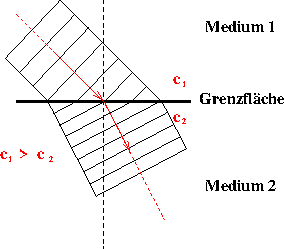
\includegraphics[width=0.5\textwidth]{build/Abb_1.pdf}
    \caption {Schematische Darstellung der Brechung einer Lichtwelle an einer Grenzfläche\cite[1]{V400}.}
    \label{fig:Abb_1}
\end{figure}
In diesem Versuch ist das zweite Medium Luft. 
Licht hat in der Luft eine Ausbreitungsgeschwindigkeit von $v_1 = c = 2,9979 \cdot 10^8 \si{\meter\per\second}$ und einen Brechungsindex von $n_1 = 1,000292$.
Somit ist $n_2$ der absolute Brechungsindex.
Ist die Ausbreitungsgeschwindigkeit vom Licht in einem Medium höher als in dem anderen Medium, 
wird es als optisch dichter bezeichnet. Ist es umgekehrt, so wird es optisch dünner genannt.
In einem homogenen Medium breiten sich die Lichtstrahlen geradlinig aus und beeinflussen sich nicht gegenseitig, selbst wenn sich zwei oder mehrere kreuzen.
Der Weg des Lichtstrahls ist umkehrbar.

\subsection{Reflexion}
\label{subsec:Reflexion}
    Wenn ein Lichtstrahl auf eine Grenzfläche trifft, wird  dieser reflektiert. 
    Es gilt das Reflexiongesetz:
    Der Einfallswinkel $\alpha_1$ ist gleich dem Reflexionswinkel $\alpha_2$.
    \begin{equation}
        \alpha_1 = \alpha_2
        \label{eqn:Reflexion}
    \end{equation}

    \begin{figure}[H]
        \centering
        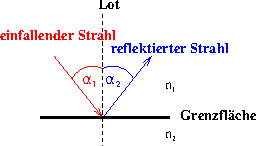
\includegraphics[width=0.3\textwidth]{build/Abb_2a.pdf}
        \caption {Reflexion eines Lichtstrahls an einer Grenzfläche\cite[2]{V400}.}
        \label{fig:Abb_2a}
    \end{figure}

\subsection{Brechung}
\label{subsec:Brechung}
    Wenn ein Lichtstrahl auf ein Medium mit einem Brechungsindex $n$ trifft, breitet er sich in diesem Medium aus. 
    Die Ausbreitungsgeschwindigkeiten in unterschiedlichen Medien sind verschieden und der Lichtstrahl erfährt an der Grenzfläche zweier Medien eine Richtungsänderung.
    Es gilt das Gesetz von Snellius(\ref{eqn:Brechung}).\\
    Falls ein Lichtstrahl durch eine planparallele Platte hindurch geht und an den beiden Grenzflächen gebrochen wird, ändert diese seine Richtung nicht.
    Er erfährt allerdings einen Strahlversatz $s$
    \begin{equation}
        s = d\frac{sin(\alpha-\beta)}{cos(\beta)},
        \label{eqn:Strahlversatz}
    \end{equation}
    welcher durch den Einfallswinkel $\alpha$, die Geometrie und das Material der Platte bestimmt wird.

    Trifft ein Lichtstrahl auf ein Prisma, welches durch nicht parallele Grenzflächen gekennzeichnet ist, wird der Lichtstrahl gebrochen.
    Der Einfallswinkel $\alpha$ ist hier für alle Wellenlängen des Lichts gleich, jedoch variiert der Brechungswinkel $\beta$. Dieser
    ist abhängig von der Wellenlänge, was als Dispersion bezeichnet wird. Weißes Licht beispielsweise wird also durch ein Prisma in seine Farben aufgeteilt.
    Die Ablenkung $\delta$, die der Lichtstrahl erfährt, wird ausgedrückt durch
    \begin{align}
        \delta = (\alpha_1 + \alpha_2)- (\beta_1 + \beta_2),
        \label{eqn:Ablenkung}
    \end{align}
    wobei die Summe der Brechungswinkel $\beta_1$ und $\beta_2$ zusammen den brechenden Winkel $\gamma$ ergibt.
    \begin{figure}[H]
        \begin{subfigure}{0,56\textwidth}
        \centering
        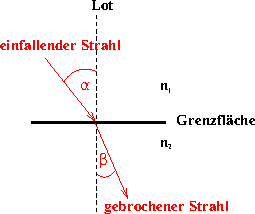
\includegraphics{build/Abb_2b.pdf}
        \caption {Brechung eines Lichtstrahls an einer Grenzfläche.}
        \label{fig:Abb_2b}
        \end{subfigure}
        \hfill
        \begin{subfigure}{0,40\textwidth}
        \centering
        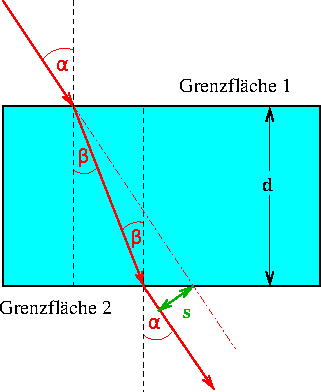
\includegraphics{build/Abb_5.pdf}
        \caption {Brechung eines Lichtstrahls an einer planparallelen Platte.}
        \label{fig:Abb_5}
        \end{subfigure}
        \caption{Brechung eines Lichtstrahls an verschiedenen Grenzflächen\cite[2]{V400}.}
    \end{figure}

\subsection{Reflexion und Transmission}
\label{subsec:R+T}
    Lichtstrahlen, die auf eine Grenzfläche treffen, werden in der Regel nicht vollständig reflektiert bzw. gebrochen.
    Ein Teil der Intensität wird reflektiert ($R$) und der andere Teil wird transmittiert ($T$) und gebrochen.
    Der Anteil der Reflexion und Transmission ist materialabhängig, es muss jedoch immer $T + R = 1$ gelten.

    \begin{figure}[H]
        \centering
        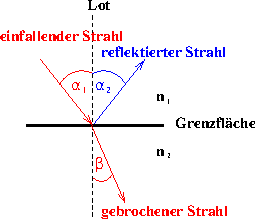
\includegraphics[width=0.3\textwidth]{build/Abb_2c.pdf}
        \caption {Brechung und Reflexion eines Lichtstrahls an einer Grenzfläche\cite[2]{V400}.}
        \label{fig:Abb_2c}
    \end{figure}

 
\subsection{Beugung}
\label{subsec:Beugung}
Wenn Licht auf ein Hindernis trifft, kann beobachtet werden, dass das Licht sich auch im Schattenbereich ausbreitet.
Die Strahlenoptik kann das Phänomen der Beugung nicht erklären, weswegen die Wellenoptik dafür benutzt werden muss.
Merkmale der elektromagnetischen Wellen sind die Frequenz $\nu$ bzw. die Wellenlänge $\lambda$ und die Ausbreitungsgeschwindigkeit $v$.
Licht besteht aus mehreren Wellenzügen.
Überlagern sich mehrere Wellen gilt das Superpositionsprinzip, die Amplituden der Wellen addieren sich also in jedem Punkt.\\
Unter der Bedingung der Kohärenz, also dass die Wellenzüge die gleiche Frequenz und eine feste Phasenbeziehung besitzen, wird ein Interferenzbild erzeugt.
Bei der Überlagerung von Wellen kann es zu einer konstruktiven Interferenz kommen, also einer  Verstärkung oder zu einer destruktiven
Interferenz, also einer Abschwächung.\\
Wenn eine ebene Wellenfront auf ein Spalt mit einer Spaltbreite $a$ trifft, werden alle Punkte an der Spaltöffnung gebeugt.
Dabei hat die gebeugte Welle die gleiche Frequenz und eine feste Phasenbeziehung.
Die Ausbreitung der Wellen wird dabei durch das Huygen'sche Prinzip beschrieben, so ist jeder Punkt einer Wellenfront der Ausgangspunkt
für eine neue Elementarwelle.
Auf einem Schirm in der Entfernung $L$, ist dann ein Muster aus dunklen und hellen Interferenzstreifen zu sehen.

